\documentclass{tex2sto}

\title{Разработка системы автоматизированного контроля документов}
\author{Иванов Иван Иванович}
\studentgroup{6401-090301D}
\institute{Институт информатики и кибернетики}
\faculty{Факультет информатики}
\department{Кафедра программных систем}
\programcode{09.03.01}
\programname{Информатика и вычислительная техника}
\studyprofile{Программное обеспечение средств вычислительной техники}
\supervisor{Петров П. П.}{доцент, к.т.н.}
\consultant{Сидорова А. А.}{консультант по экономике}
\normcontroller{Кузнецова Н. Н.}
\city{Самара}
\year{2026}

\assignmentvariant{2}
\assignmentapprover{заведующий кафедрой П. И. Сергеев}
\assignmentgoal{разработать воспроизводимый способ контроля оформления документов}
\assignmentquestions{проанализировать требования; разработать модель; проверить результаты}
\assignmentissued{01.02.2026}
\assignmentdue{01.06.2026}

\keywords{ДОКУМЕНТ; КОНТРОЛЬ; МОДЕЛЬ; ВАЛИДАЦИЯ; АВТОМАТИЗАЦИЯ}
\begin{abstract}
Разработана система автоматизированного контроля документов. Определены ограничения
входного языка, реализованы проверка структуры и формирование редактируемого документа.
Эксперимент показал воспроизводимость результатов при использовании единого профиля.
\end{abstract}

\source{sto}{standard}{}{СТО 02068410-004-2018}{Самара: Самарский университет, 2019. 37 с.}
\source{pandoc}{web}{Pandoc contributors}{Pandoc User's Guide}{URL: https://pandoc.org/MANUAL.html (дата обращения: 09.09.2026)}

\begin{document}

\definitions
\definition{Документ}{результат компиляции исходного текста в целевой формат}

\abbreviations
СТО --- стандарт организации.

\introduction
Оформление работы должно быть воспроизводимым. Требования стандарта~\cite{sto}
используются как нормативная основа. В приложении~\ref{app:code} приведён пример кода.

\section{Анализ требований}
\subsection{Ограничения входного языка}
Поддерживается контролируемый диалект. Он включает:
\begin{itemize}
\item семантические команды документа;
\item вложенные списки:
  \begin{enumerate}
  \item первый проверяемый элемент;
  \item второй проверяемый элемент.
  \end{enumerate}
\end{itemize}

Архитектура решения показана на рисунке~\ref{fig:architecture}.
\begin{figure}
\centering
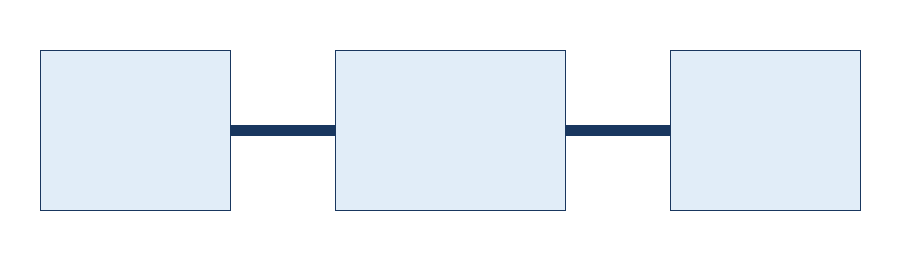
\includegraphics{architecture.png}
\caption{Архитектура конвейера преобразования}
\label{fig:architecture}
\end{figure}

\section{Модель и реализация}
Критерий~\ref{eq:quality} связывает число пройденных проверок с общим числом проверок:
\begin{equation}
Q = \frac{N_{passed}}{N_{total}}
\label{eq:quality}
\end{equation}
где $Q$ --- доля пройденных проверок; $N_{passed}$ --- число успешных проверок;
$N_{total}$ --- общее число проверок.

Результаты представлены в таблице~\ref{tab:results}.
\begin{table}
\caption{Результаты проверки}
\label{tab:results}
\begin{tabular}{|l|l|}
\hline
Формат & Результат \\
\hline
DOCX & пройдено \\
PDF & пройдено \\
\hline
\end{tabular}
\end{table}

Полный журнал приведён в таблице~\ref{tab:log}. Таблица допускает продолжение
на следующей странице с повтором строки заголовка.
\begin{longtable}{|l|l|}
\caption{Журнал проверок}
\label{tab:log}\\
\hline
Проверка & Состояние \\
\hline
Структура & пройдено \\
Стили & пройдено \\
Поля & пройдено \\
Формулы & пройдено \\
Ссылки & пройдено \\
\hline
\end{longtable}

Реализация использует проверенный маршрут преобразования~\cite{pandoc}.

\conclusion
Разработана первая версия системы. Она формирует редактируемый DOCX и независимый PDF,
а также сообщает о нарушениях контролируемого диалекта.

\printbibliography

\appendix{app:code}{Пример программного кода}
\begin{verbatim}
def check_document(source: str) -> bool:
    return bool(source.strip())
\end{verbatim}

\end{document}
